	Our proposed \gls{cawi} system uses the \gls{rest} architecture \cite{phdthesis:fielding00} to consider architectural principles such as scalability, simplicity or reliability. Through \gls{rest}, the system is constrained to produce uniform interfaces using the \gls{http} verbs (e.g. GET, POST, PUT and DELETE). This restriction permits client and server to \emph{evolve} independently. For instance, changes at any service implementation reduce or eliminate the impact produced on the client. The stateless constraint, also from \gls{rest}, requires to have a server solution that avoids keeping session state for each client. For that restriction, we have implemented a token based identifier that makes it easier to \emph{scale} our solution without needing to replicate any session data across a multi-server configuration. Reliability is improved because it eases the task of recovering from partial failures within components, connectors or data \cite{phdthesis:fielding00}.

	The system is structured to separate the \gls{cawi} services from the user interfaces (see Figure \ref{fig:design:architecture}) using \gls{json} and \gls{xml} standard exchange data formats for communication. 
	%Look at which part of the architecture is driven by CAWIML. You need to find away to illustrate that on the figure and explain it when at first mention of the figure.
	The server side is structured into different layers: 
	\begin{itemize}
		\item the \emph{\gls{api} layer} (e.g. RESTful API), that uses the \gls{http} methods defined by RFC 2616 \cite{web:fielding99} creates the communication interfaces and is the only component that is directly accessible by the client;
		\item the \emph{business layer}, used by the \gls{api}, separates the different functionalities of the system through Java packages (e.g. content, routing, personalisation) in order to promote reusability; and
		\item the \emph{data access layer}, which serves to abstract the data storage solution from the business layer, makes the system easier to maintain since this connector is centralised in one place.
	\end{itemize}

	This layered server structure induces \emph{portability}, thanks to the use of Java as the general purpose programming language that works across any platform.

	\begin{figure}[h]
	\centering
	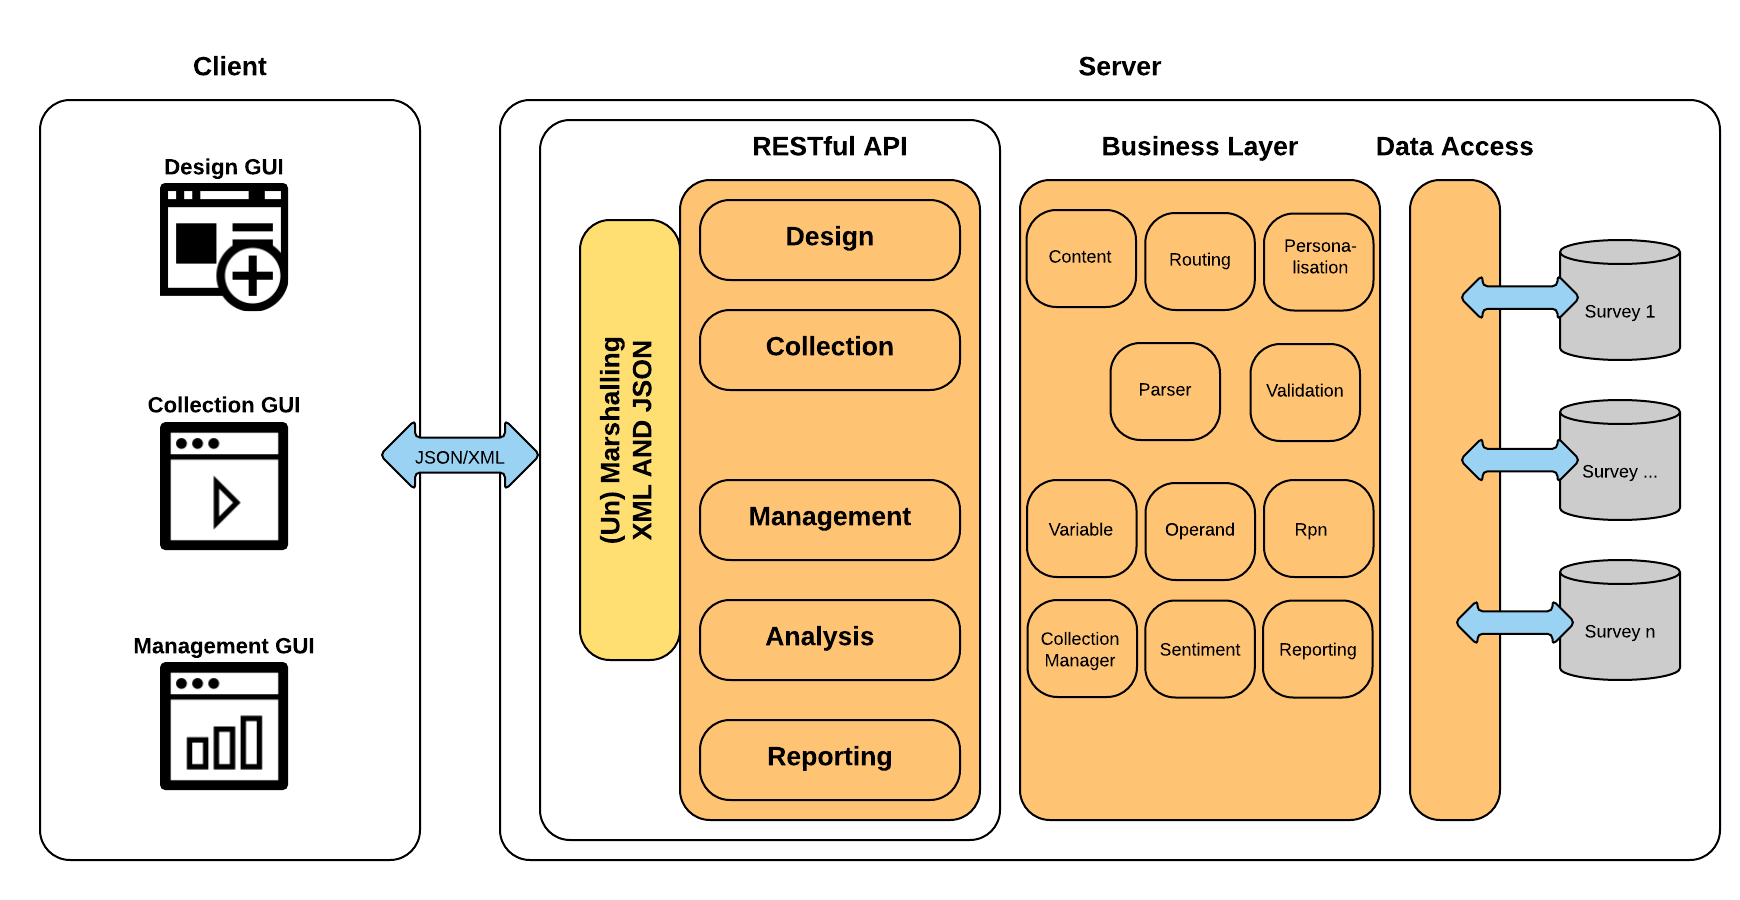
\includegraphics[max size={\textwidth}{\textheight}]{design/img/surveyArchitecture.png}
	\caption{REST architecture}
	\label{fig:design:architecture}
	\end{figure}

	The client side of this architecture makes a clear separation by building and rendering every \gls{html} code entirely on the client using the novel \gls{spa} paradigm (see Section \ref{sec:cawiSystem:spa}). This approach when compared to the multi-page paradigm, that Blaise or SurveyMonkey adopt, is more consistent with the \emph{simplicity} property, since it reduces the amount of data transferred from the server, improves user experience and reduces the burden on the server.
